% to choose your degree
% please un-comment just one of the following

\documentclass[bsc,frontabs,twoside,singlespacing,parskip,deptreport,logo]{infthesis}     % for BSc, BEng etc.
% \documentclass[minf,frontabs,twoside,singlespacing,parskip,deptreport]{infthesis}  % for MInf


\usepackage{tikz}
\usetikzlibrary{timeline}


\usepackage{graphicx}
\usepackage{url}
\usepackage{amsmath}
\usepackage{caption}
\usepackage{subcaption}
\usepackage{gensymb}
\usepackage[capposition=bottom]{floatrow}


\graphicspath{ {Pictures/background/}{Pictures/models/}{Pictures/elastica/}{Pictures/illusions/}{Pictures/experiments/rnn/} {Pictures/experiments/exp1_fig2/} {Pictures/experiments/fig5/} {Pictures/experiments/fig5/figB}}



\newcommand{\plottwofigures}[4]{
\begin{figure}[H]
\centering
\begin{subfigure}{.5\textwidth}
  \caption{}
  \centering
  \includegraphics[width=.8\linewidth]{#1}
\end{subfigure}%
\begin{subfigure}{.5\textwidth}
  \caption{}
  \centering
  \includegraphics[width=.8\linewidth]{#2}
\end{subfigure}
\caption[#4]{#3}
\label{#1}
\end{figure}
}


\newcommand{\plottwofiguresS}[5]{
\begin{figure}[H]
\centering
\begin{subfigure}{.5\textwidth}
  \caption{}
  \centering
  \includegraphics[width=#5\linewidth]{#1}
\end{subfigure}%
\begin{subfigure}{.5\textwidth}
  \caption{}
  \centering
  \includegraphics[width=#5\linewidth]{#2}
\end{subfigure}
\caption[#4]{#3}
\label{#1}
\end{figure}
}


\newcommand{\plotfigure}[3]{
\begin{figure}[H]
\centering
\includegraphics[width=.8\linewidth]{#1}
\caption[#3]{#2}
\label{#1}
\end{figure}
}


\newcommand{\plotfigureS}[4]{
\begin{figure}[H]
\centering
\includegraphics[width=#4\linewidth]{#1}
\caption[#3]{#2}
\label{#1}
\end{figure}
}

\newcommand{\plotthreefigures}[6]{
\begin{figure}[H]
\begin{subfigure}{.33\textwidth}
  \centering
  \includegraphics[width=#6\linewidth]{#1}
  \caption{}
\end{subfigure}%
\hfill
\begin{subfigure}{.33\textwidth}
  \centering
  \includegraphics[width=#6\linewidth]{#2}
  \caption{}
\end{subfigure}
\hfill
\begin{subfigure}{.33\textwidth}
  \centering
  \includegraphics[width=#6\linewidth]{#3}
  \caption{}
\end{subfigure}%
\label{#1}
\caption[#5]{#4}
\end{figure}
}

\newcommand{\plotfigures}[5]{
\begin{figure}[H]
\caption{}
\begin{subfigure}{.5\textwidth}
  \caption{}
  \centering
  \includegraphics[width=1\linewidth]{#1}
\end{subfigure}%
\begin{subfigure}{.5\textwidth}
  \caption{}
  \centering
  \includegraphics[width=1\linewidth]{#2}
\end{subfigure}
\begin{subfigure}{.5\textwidth}
  \caption{}
  \centering
  \includegraphics[width=1\linewidth]{#3}
\end{subfigure}%
\begin{subfigure}{.5\textwidth}
  \caption{}
  \centering
  \includegraphics[width=.1\linewidth]{#4}
\end{subfigure}
\label{#1}
\floatfoot{#5}
\end{figure}
}

\newcommand{\plotfiguresix}[9]{
\begin{figure}[H]
\centering
\begin{subfigure}[b]{#8\textwidth}
  \centering
  \includegraphics[width=\textwidth]{#1}
  \caption{}
\end{subfigure}
\hfill
\begin{subfigure}[b]{#8\textwidth}
  \centering
  \includegraphics[width=\textwidth]{#2}
  \caption{}
\end{subfigure}
\hfill
\begin{subfigure}[b]{#8\textwidth}
  \centering
  \includegraphics[width=\textwidth]{#3}
  \caption{}
\end{subfigure}
\hfill
\begin{subfigure}[b]{#8\textwidth}
  \centering
  \includegraphics[width=\textwidth]{#4}
  \caption{}
\end{subfigure}
\hfill
\begin{subfigure}[b]{#8\textwidth}
  \centering
  \includegraphics[width=\textwidth]{#5}
  \caption{}
\end{subfigure}
\hfill
\begin{subfigure}[b]{#8\textwidth}
  \centering
  \includegraphics[width=\textwidth]{#6}
  \caption{}
\end{subfigure}
\caption[#9]{#7}
\label{#1}
\end{figure}
}

\newcommand{\plotfiguresixn}[7]{
\begin{figure}[H]
\caption{}
\begin{subfigure}{.5\textwidth}
  \centering
  \includegraphics[width=.8\linewidth]{#1}
\end{subfigure}%
\begin{subfigure}{.5\textwidth}
  \centering
  \includegraphics[width=.8\linewidth]{#2}
\end{subfigure}
\begin{subfigure}{.5\textwidth}
  \centering
  \includegraphics[width=.8\linewidth]{#3}
\end{subfigure}%
\begin{subfigure}{.5\textwidth}
  \centering
  \includegraphics[width=.8\linewidth]{#4}
\end{subfigure}
\begin{subfigure}{.5\textwidth}
  \centering
  \includegraphics[width=.8\linewidth]{#5}
\end{subfigure}%
\begin{subfigure}{.5\textwidth}
  \centering
  \includegraphics[width=.8\linewidth]{#6}
\end{subfigure}
\label{#1}
\floatfoot{#7}
\end{figure}
}

\newcommand{\bt}[1]{
\textbf{#1}
}

\newcommand{\eq}[1]{
\begin{equation}
  {#1}
\end{equation}
}

\newcommand{\eql}[2]{
\begin{equation}
  {#1}
  \label{#2}
\end{equation}
}
\begin{document}

\title{Visual illusions and interactions in biologically inspired neural networks. Analyzing perception of tilt}

\author{Martin Andreev Asenov}

% to choose your course
% please un-comment just one of the following
\course{Artificial Intelligence and Computer Science}
%\course{Artificial Intelligence and Software Engineering}
%\course{Artificial Intelligence and Mathematics}
%\course{Artificial Intelligence and Psychology }   
%\course{Artificial Intelligence with Psychology }   
%\course{Linguistics and Artificial Intelligence}    
%\course{Computer Science}
%\course{Software Engineering}
%\course{Computer Science and Electronics}    
%\course{Electronics and Software Engineering}    
%\course{Computer Science and Mathematics}
%\course{Computer Science and Physics}  
%\course{Computer Science and Statistics}    

% to choose your report type
% please un-comment just one of the following
%\project{Undergraduate Dissertation} % CS&E, E&SE, AI&L
%\project{Undergraduate Thesis} % AI%Psy
\project{4th Year Project Report}

\date{\today}


\abstract{
We experience different tilt illusions and pop out effects. This is often explained by the line's representation in the visual cortex. A group of neurons is responsible for detecting different orientations in different parts of our visual field. A neuron tuned for a specific orientation spikes more, when its preferred orientation is presented, and less the more different the orientations is, forming a bell shaped curve of activity. We have multiple neurons for every part of our visual field, tuned for different orientations. Combining their responses we get an accurate response of the actual orientation, despite their noisy spiking.

However neurons responsible for different part of our visual field are also connected to each other. This modulation explains some of the effect we are experiencing, as orientations in our visual fields are influenced by nearby ones. However those interaction have only been explored statically, calculating the modulation only once. In a full dynamic a change in an orientation, can lead to a change in another orientation, and so on. It's unclear if existing models change in a dynamic setting, does the system settles down to a stable state, or it keeps fluctuating.

In this report, we explore an already existing passive model of the above mentioned neurons and build a dynamic model. We explore the differences between the two to check if in a dynamic setting, we still experience the same effects. 
}

\maketitle

\section*{Acknowledgements}
Acknowledgements go here. 

\tableofcontents
\listoffigures
%\listoftables

%\pagenumbering{arabic}


\chapter{Introduction}

In processing visual information, our brain seems to favor continuity and prioritize the greater whole, rather than individual details. Sometimes this ability serves us well, ex. when trying to find a pattern among random noise, or a discontinuity in a certain pattern (fig.\ref{popout}). However in other cases this leads to various illusions (fig.\ref{illusion1}, fig.\ref{illusion2}). The project aims to explore the relevance of V1 and its orientation selectivity neurons in the context of those effects. Fig.\ref{illusion1} and fig.\ref{popout} are particularly relevant to this project.

This paper develops a model, based and built upon the one described in the recent elastica paper \cite{keemink2015unified}. The elastica principle defines the strength of the connections between different orientation selective neurons. It favors continuity, the smoother too bars are connected to each other, the stronger the modulation connection between them. Although there are other models explaining similar phenomena, illusions and effects separately, the neural model described claims to have all of those properties, unifying them in one model. 

However all the results obtained were obtained statically with only one pass through the model. As mentioned in further development, adding dynamics to some of the already presented illusions could lead to some interesting behavior. We build a recurrent neural network of the orientation selective neurons in the V1 cortex. We set the strength of the connections between them (weights in the network), based on the elastica principle. We perform baseline experiments with the static model and compare the results in full dynamic setting.

The different parts of the project are discussed below in the report.
\begin{itemize}
  \item Background - gives some necessary neuroscience terminology and information about the problem and concepts we are going to use. We also briefly discuss recurrent neural networks, as they are the model used for simulating experiments.
  \item Design - discuss the design of the experiments and the evolution of the model, before the final version used for running experiments.
  \item Implementation - choice of programming languages and libraries, why they are important to the project and how they influence both the speed and ease of running experiments, but also the workflow of conducting research.
  \item Experiments - in depth description of experiments ran
  \item Evaluation - comparing the results gathered from experiments
  \item Timeline - timeline of the work done through the project.
  \item Conclusions - final conclusions
\end{itemize}



\plotfigure{illusion1}{The orientations of the small circles inside seem tilted \cite{baggott2010investigating}}{Tilt illusion}
\plotfigureS{illusion2}{The lines do not seem parallel, when it reality they are \cite{vision-computation}}{Parallel illusion}{.5}
\plotfigureS{popout}{The central bar is easily detected by our vision system, due to the difference from the nearby orientations}{Pop out effect}{.3}


\chapter{Background}

In explaining the model setup and performed experiments, it is important to first introduce some neuroscience terminology. As one can imagine the visual cortex is utterly complex. We are focusing on the V1 cortex, analyzing a specific type of orientation selective neurons. Even though we are focusing on a specific neurons in only a part of our visual processing pipeline, we make even more simplifications in order to be able to analyze specific features of those neurons. We also briefly introduce recurrent neural networks and how they are used in the project.

\section{Neuroscience background}
\subsection{Visual field and visual stimuli}

Visual field is the area we can see with our eyes. The information undergo a variety of transformations in the different parts of our visual cortex. The first few processing steps are illustrated in fig.\ref{visual_fields}. The initial information we receive is changes in light from our retina. This then gets processed by the lateral geniculate nucleus (LGN). The LGN cells  and passed down to the Primary visual cortex (V1). V1 extract information about edges and orientations in the different parts of our visual field. 

\plotfigureS{visual_fields}{Perceiving a line from the retina to LGN cells and then by V1 orientation selective cells.\cite{receptive-fields}}{Visual Field}{.5}

Precisely how this information is processed is the main interest of this project. While at a retinal and LGN level, most of the transformations are low-level, V1 starts to extract some patterns. We don't only detect single orientations for different parts of our visual field. Nearby orientations can influence each other. 

(to rewrite)
Nearby orientations of the orientations useful for the high level visual processing happening in V2, V3, V4, V5 and V6. 

mention visual stimuli

Finally it is also worth mentioning that we see in different details in different parts of our visual fields. Most of the information we perceive is close to the central or foveal vision, which could lead to interesting behavior \cite{knight2008drastically}. A small part of our retina, known as 'blind spot', does not have any photoreceptors. Our brain compensates the lack of information by fulfilling details from nearby observations. Both of those details could lead to change in behavior in our model, however we will ignore this details in our experiments.

\plotfigure{RetinotopicMapping}{\bt{Central and peripheral vision}\cite{retinotopic-mapping} Substantial number of the cells in the retina are devoted to only a small part of our visual field, or central vision. Although relevant to the project, we will ignore this detail, for the benefit of simpler model}{Central and peripheral vision}

\subsection{Receptive fields}

In general, a receptive field is defined as a region of the sensory space, which can stimulate a given sensory neuron. In our context we can define the receptive field of a neuron, as the part of visual field, which affects it \cite{Hartline700}. The above two definition are known as classical receptive fields.

It was later discovered that time plays a role as well, making the definition more complicated \cite{deangelis1995receptive}. In our model, described later, we focus on the spatial and ignore the temporal separation of receptive fields. Moreover because neurons are connected to each other, the notion of receptive field can get a bit vague. Because of those connection a neuron, can get excited or inhibited from parts of the visual field, that the neuron is not directly connected to (fig.\ref{F4large}).

To avoid confusion we will stick to the definition of classical receptive fields, and distinguish between the input a neuron receives because of its tuned orientation and modulation from nearby neurons.

\plotfigureS{F4large}{\bt{Effect of the context on receptive field on a neuron}\cite{cavanaugh2002nature} The firing of neurons is indirectly modulated and their response shifted, based on the stimuli just outside of their receptive field. This leads to some of the complications of explaining receptive field. Even though a certain neuron is tuned for only a certain part of our vision field, for certain orientation, it can be affected by nearby neurons. If we take this to the extreme, then a receptive field is based on all the sensory input we receive, since one neuron excites a nearby one, which excites its nearby neurons, etc.}{Effect of the context on receptive field on a neuron}{.5}

\subsection{Tuning curves}

Different orientation selective neurons are tuned for different orientation at a specific part of the visual field, defined by their receptive field. In other words neurons like specific orientation place at a specific place. However they spike not only when the preferred orientation is presented, but also on similar to its preferred orientation. The intensity of spiking, when different orientations are presented, forms a bell shaped curve with a peak the preferred orientation of the neuron. 

\plotfigure{HubelWiesel}{\bt{Tuning curves}\cite{hubel1968receptive} Different orientation bars are presented in a certain part of the visual field(on the left), and the response of the neuron tuned for this specific part of the visual field and $0\degree$. Even though the neuron is tuned for $0\degree$, its spikes when similar orientations are presented. The closer the orientation is to its preferred one, the stronger the response.}{Tuning curves}


\subsection{Population coding}

We have multiple orientation selective neurons per part of our receptive field. They all spike with different intensity defined by their tuning curves. Our final perception of the orientation in that part of the visual field is based on the all the spiking of the neurons. Their preferred orientation and magnitude can form a vector, with direction based on the preferred orientation and length based on the magnitude. When the vectors are added together, we get the final perceived orientation, with magnitude, as before, the length of the vector and perceived orientation - the direction of the vector.

\plotfigure{populationCoding}{\bt{Population coding in the motor cortex}\cite{amirikian2000directional} Although the above picture illustrates population coding in a different part of the brain, it still good illustration of population coding. Different orientation selective neurons respond with certain intensity (black bars) and their response are combined to show the final perceived perception(red bars).}{Population Coding}

\section{Elastica principle}

The elastica principle defines the strength of modulation between two neurons. We find the smoothest curve connecting the two bars. The elastica energy is then defined by the length of the curve. The smoother curve they form, the more strongly they should be connected. The principle is illustrated in fig.\ref{elastica1}.

\plotfiguresix{elastica1}{elastica5}{elastica3}{elastica4}{elastica2}{elastica6}{\bt{Elastica principle} (to include energies for all curves) a) 0 b) ...}{.3}{Elastica principle}




\section{Recurrent Neural Networks}

A recurrent neural network (RNN) is a type of neural network with two way connections between its neurons. The benefit compared to a standard feedforward architecture is that can model dynamic behavior, where the responses of neurons change with respect to time. The network settles in a stable state, periodic or chaotic behavior. Two problems with RNNs are training and the expensive simulation of small timesteps. However they are not an issue as we set the weights based on the elastica principle and the experiments we run are on relatively small visual fields.

\chapter{Design}

This paper implements simplified versions of visual field, receptive fields, tuning curves and population coding in a recurrent neural network with orientation selective neurons. We start with a simple model with one receptive field, extend the model to multiple receptive fields, define limited and full connectivity and finally implement the elastica principle as well. In this section the different models are described in detail. In designing the model, I decided to use iterative and incremental development. The simplest models were mostly used for validity checks, rather than any meaningful experiments. Most of the experiments were based on the final version of the model, with full connectivity with weights setup according to the elastica principle.  

The input our model receives is a matrix of numbers from the interval $0-1$, representing different orientation from $0\degree$ to $180\degree$. The output has the same form and represents what orientations the model perceives. Fig.\ref{input_random} shows a visualization of a sample input to the model. It's important to note that the model returns not only a single matrix with perceived orientations, but multiple ones, representing the state at different timesteps.


\plottwofigures{input_random}{input_structure}{\bt{Visualization of sample input(output) to the model} (A) Random orientations. (B) All orientations from $0\degree$ to $180\degree$, for every $1.8\degree$.}{Sample input}

For every orientation of the input (every bar in fig.\ref{input_random}), we have a stack of neurons tuned for different orientations. Fig.\ref{stacked_neurons3} illustrates this. The perceived orientation is affected from two factors. 

First of all to detect a specific orientation, we have a stack of different neurons tuned for different orientations (fig.\ref{stacked_neurons3}, (A)). They all spike with different intensities and their collective response, forms the perceived orientation. 

Secondly, every single orientation orientation in our visual field, has its own stack of neurons (fig.\ref{stacked_neurons3}, (B)). Based on all those neurons, we can get accurate information about all the orientations (the higher the number of neurons used, the more accurate the perceived orientation is).

The complexity comes from the fact that the different 'stacks of neurons' are connected with the nearby stacks. Those connections and how they influence the perceived orientation in a dynamic setting is the main focus of experiments ran.

\plottwofigures{stacked_neurons3}{stacked_neurons2}{\bt{Visualization of the orientation selective neurons and their relationship with the presented input.} (A) Presented orientation(left) and responses of the orientation selective neurons(right). The more saturated the color, the stronger the response is. The neurons will spike with higher intensity, depending on the difference of the presented orientation and their preferred orientations. All the responses are combined, giving the final perceived orientation. (B) Schematic representation of the input and orientation selective neurons. Every orientation bar has its own stack of orientation selective neurons (only the first few are shown).}{Overview of the model}

\plottwofiguresS{stacked_neurons}{neuron2}{\bt{Two different visualizations of orientation selective neurons} A) Visualization of 6 neurons in a stack form B) 9 orientations in unrolled form. Both of the visualization are for purely illustrative purposes. Visualization A) is used to explain the general model, while visualization B) better explains the connections between the neurons.}{Stack of neurons}{.3}


\section{Single orientation}

First we implement a visual field with a single orientation. We have a couple of neurons responsible for detecting the orientation (fig.\ref{stacked_neurons}).

As described in \cite{keemink2015unified}, we represent those responses as vectors, with direction their preferred orientation and magnitude, the strength of the response with respect to the stimuli. Summing those vectors gives us the perceived orientation. Although used for recording responses from different types of neurons, fig.\ref{populationCoding} shows how population coding works. Black vectors are neural activity from specific neurons, and the red vector is the sum of all those responses.

Even at this small scale, some experiments (described later) can be run, which show the relation between number of orientation selective neurons used and the accuracy of the perceived orientation.

\section{Two orientations}

Next we extend the model so we can feed two orientations and we have orientation selective neurons for the two orientations. We add recurrent connection between the neurons with the same preferred orientations, as showed in fig.\ref{neuron5}, (A), (B). This adds contextual modulation, as the perceived orientation of a single orientation in the visual field is influenced by the other one.

The firing rate of the pairs of same orientation selective neurons in the two visual fields is calculated by the differential equations:

\begin{equation}
\label{model11}
\tau_{syn}\cfrac{dr_{1}(t)}{dt}=-r_{1}(t)+in_{1}+w_{12}r_{2}
\end{equation}


\begin{equation}
\label{model12}
\tau_{syn}\cfrac{dr_{2}(t)}{dt}=-r_{2}(t)+in_{2}+w_{21}r_{1}
\end{equation}

where $\tau_{syn}$ is a constant, $\cfrac{dr_{1/2}(t)}{dt}$ is the change of the firing rate with respect to time, $r_{1/2}(t)$ is the current firing rate, $w_{12/21}$ is the strength between the neurons. $in_{1/2}$ is calculated from the tuning curve of the specific neuron for the  presented orientation. In our model we will use the von Mises function as in \cite{keemink2015unified}. The von Mises function has the following formula:

\eq{A\exp(k\cos2(\alpha_{pref} - \alpha_{actual}))}


The different values of $A$ and $k$ are again described in \cite{keemink2015unified}, but ultimately the function with the correct set of parameters gives us the similarly looking tuning curves as in fig.\ref{HubelWiesel}.

Finally to calculate the perceived orientations in the visual field by adding all responses from each part of the visual field as vectors. The direction of a vector is the preferred orientation of the given neuron, and the length is the magnitude of the response. Since the preferred orientation are direction independent, they vary from $0$ to $\pi$. As described in \cite{keemink2015unified}, to ensure circularity, we multiply all the responses by $2$, add them together and divide them by $2$ at the end.

\eq{\alpha_{perceived}=\cfrac{1}{2}\sum_{i}2\vec{r}_{i}}


%\plottwofigures{neuron5}{neuron3}{\bt{Two orientations, with limited connectivity between neurons}}

\section{Multiple orientations, limited connectivity}

Next we extend the model, so we can have any number of orientations (fig.\ref{neuron1}). Every neuron (except the ones at the end at the visual field) is connected with the eight closest neurons, which have the same preferred orientation as his (fig.\ref{neuron1}). We can extend the formulas \ref{model11} and \ref{model12} to:

\begin{equation}
\tau_{syn}\cfrac{dr_{i}(t)}{dt}=-r_{i}(t)+in+\sum_{j} w_{ij}r_{j}
\end{equation}

 
\plotfigureS{neuron1}{\bt{Any number of orientations, with limited connectivity between neurons} *The connections for only one neuron are shown.}{Limited connectivity}{0.7}

\section{Multiple orientations, full connectivity} \label{mult_model}
The next modification we do, on single neuron level, is to add full connectivity between all the neurons. We set the weights depending on the closeness of the neurons to each other, as well as the similarity of their preferred orientation. To explain how we setup the weights, let use an example. Let's have a $10x10$ visual field with different orientations, as in fig.\ref{input_random} and $9$ orientations selective neurons. Unrolling the $10x10x9$ matrix, we have a vector of $900$ neurons all together. We can setup $900x900$ weight matrix defining the connections between the neurons. 

Having some distance and the orientation constants as $\kappa_{distance}$ and $\kappa_{orientation}$, for every two neurons $l$ and $m$, we model the strength of the connection between them as:

\eq{d=\sqrt{{(i_{l}-i_{m})}^{2}+{{(j_{l}-j_{m})}^{2}}}}

\eq{\delta=min(mod(\alpha_{l}-\alpha_{m},1),mod(\alpha_{m}-\alpha_{l},1))}

\eql{w_{i,j}=w_{j,i}=\kappa_{distance}\cfrac{1}{exp(d)} + \kappa_{orientation}\cfrac{1}{exp(\delta)}}{mult_model_formula}


Based on the above equations we have the updating of the network as:

\begin{equation}
\tau_{syn}\cfrac{dr_{i}(t)}{dt}=-r_{i}(t)+in+\sum_{j=0}^{\#neurons}w_{ij}r_{j}
\end{equation}

We can vectorize our equation (and code), so we have:

\begin{equation}
\tau_{syn}\cfrac{dr_{i}(t)}{dt}=-r_{i}(t)+in+Wr
\end{equation}

The strength of the connection between every two neurons $l$ and $m$ is the same as the recurrent connection between $l$ and $m$, so the matrix is symmetric with respect to the main diagonal. The values along the main diagonals are $0$ (a neuron does not have a connection with itself). We can also notice the general trend of having highest values along the main diagonal and then smaller values the further away we go. This is true for different scales of our matrix - the full matrix (a), the first $100x100$ square (b) as well as the first $10x10$ square (c). The three different scales represent the change in orientation, horizontal and vertical position.



\plotthreefigures{weight1}{weight2}{weight3}{Weight matrix for a full connectivity model. (A) Full weight matrix. (B) First 100 neurons. (C) First 10 neurons. (D) Scale of the values.}{Sample weight matrix}{1}

\section{Elastica principle}

The final part is implementing the elastica principle into the model. The only modification we have to do in comparison to the full connectivity model (sec.\ref{mult_model}) is change the equation calculating the weights, or the strength between respective neurons. In the previous model, we were setting based on the difference of the preferred orientations of the two neurons and the distance between them (eq.\ref{mult_model_formula}).






\chapter{Implementation}

This sections discusses the choice of programming languages and libraries, the benefits and challenges of using them and how they were addressed. During the implementations stages, I went through variety of changes, depending on the current stage of the project. First versions of visual fields, receptive fields, tuning curves and population coding were implemented. Next we implement a model of the input the orientation selective neurons in our V1 cortex receive and how the neurons respond to it. We gradually extend our model, to include more options for changing the connections between two neurons, as well as the form on the input. We use different tools for visualization and address some performance issues of simulating the model and running different experiments.


\section{Initial choice of programming language}
My first choice of programming language was Matlab. Matlab is a high-level scripting language, highly optimised for linear algebra operations. It is a well suited language for the purposes as it takes a lot of the complexity of memory management, parameter passing, multiple memory spaces, etc, of language like C++ has for example. As matrices and vectors additions and multiplications were the main bottle neck in this project, Matlab provided the necessary performance, while being simple and convenient to use. Moreover as most of the functions in Matlab can receive as an input a single number, vector or matrix, the model we built can be easily extended and tested for different configurations. Their integrated IDE with interpreter, standard debugging tools (breakpoints, continue, step in/out, etc.), workspace of current variables in scope, provided additional convenience in the initial stage of development.

\section{Model implementation}
I implemented versions of visual stimuli orientations selective neurons in V1 receive, tuning curves and population coding. The visual stimuli was implemented as a field of different bars (or edges, lines) of particular orientation, so a matrix with numbers from $0$ to $\pi$. The tuning curve of a particular neuron is defined as the spike activity when a particular orientation is presented, as a function of its preferred orientation. As mentioned in the previous section most of the functions in Matlab accept numbers, vectors and matrices as their arguments. This makes in particularly useful, as the function can be implemented for a single neuron, tested for expected output, and then the function can be used for vectors or matrices, when running more complicated experiments. As mentioned in the background section, we receive output from different orientation selective neurons  about a particular bar of orientation. We use population coding to add their responses to get the final, perceived orientation. We implement population coding by transforming the output of the neurons in vectors. The preferred orientation of every neuron is the direction of the vector, the magnitude of its spiking is the length of the vector. We add all the vectors together to get a new vector, which represents the perceived orientation. The final vector's length and direction represent respectively the magnitude orientation of the final perceived response. As the orientation bars vary from $0$ to $\pi$, we multiply by $2$ the direction of all the neurons, and divide the final direction by $2$, to ensure circularity.
We gradually extended the form on the input from a single orientation bar, to two and multiple ones in a form of matrix. We also extend the modulation connections between different neurons. Along different implementations we take advantage of the optimized linear operations in Matlab, and we keep our code vectorized, rather than for loops (with the exception of simulating different time steps of interactions between neurons, as the next state depends on the previous one).

\section{Change of development tools}
As the work progressed it became clear that Matlab, may not be the best choice of programming language for the project. After running some initial experiments, issues started coming up, which lead to transition to different set of programming tools, which we used for the final experiments. In our model we have different orientations bars, with a group of orientation selective neurons spiking for each bar and influencing the spiking of nearby neurons. It is a high dimensional data, hard to visualize. Moreover as we have dynamic interactions, implement by a recurrent neural network, we have the above mentioned data for every time step of our simulation. As the project grew bigger, some of the disadvantages of the weak code organization of Matlab became apparent, making hard to keep all the code base well structured.

After careful consideration I decide to rewrite the work I've done in Python taking advantage of libraries like Holoviews\cite{stevens2010holoviews}, Matplotlib\cite{hunter2007matplotlib} and Numpy. I also started using IPython notebooks\cite{shen2014interactive}. Although the transition process took a couple of weeks, it yield number of advantages outlined below.

\textbf{Python}
\begin{itemize}
  \item Scalability - every function can be easily extended, by adding a new parameter and setting a default value, so it does not change the previous behaviour of the function
  \item Compatibility - Python is compatible with number of useful libraries, some of which used are described below
  \item Link to previous work - I took advantage of some of the code base of \cite{keemink2015unified}. In particular I used the methods for calculating and visualizing the elastica energy.
\end{itemize}

\textbf{Holoviews}
\begin{itemize}
	\item Interactive visualizations - building complex interactive visualization, with respect to any number of parameters. In case of our problem, we used it for visualization of perceived orientation with respect to time
\end{itemize}

\textbf{Matplotlib}
\begin{itemize}
	\item Main tool for static plots - although Holoviews provides some really advanced plotting capabilities, its API is sometimes complicated and tedious to use. Matplotlib is much widely used libraries with rich documentations and examples online.
\end{itemize}

\textbf{Numpy}
\begin{itemize}
	\item Numerical operations - Numpy provides number of mathematical operations as well as functions for matrices and vectors manipulation. In addition its syntax is almost identical to Matlab, speeding up the transition process.
\end{itemize}

\textbf{IPython Notebook}
\begin{itemize}
	\item Reproducible research - experiments can be specified and ran in a notebook. Results are shown under every experiment, also giving the option to run part or all of them again.
	\item Documenting - support from markdown cells (in addition to the code cells for the experiments) with rich formatting, including support for LaTeX.
\end{itemize}

Using the above stack of software tools greatly improved not only the development process, but also conducting and documenting experiments.

\section{Final model changes}
After transitioning to Python I incorporated the elastica principle in my model. Give two orientations selective neurons, the elastica principle defines how strongly they should be connected, by calculating their elastica energy.

I also extended my model to custom positions of the neurons, rather than the fixed matrix grid. Rather than calculating the locations of the orientations, based on their position in the matrix, one can use a $1xN$ vector to represent all the neurons orientations together with $2xN$ matrix to represent their locations. This allows us to reproduce most of the experiments in \cite{keemink2015unified}, in the dynamic setting of the model. For some of the bigger experiments we run, we also implement a torus for the connections between the neurons.


\chapter{Experiments}

\section{Recurrent Neural Network}

First we explore a simple network with only one neuron. The neuron receives a certain excitation ($in$). The speed with which the neuron changes it's response, depends on the contant $\tau_{syn}$ (the smaller $\tau_{syn}$, the slower the change). We setup the simple recurrent neural network below.

\eq{\tau_{syn}\frac{dr(t)}{dt}=-r(t)+in}

So every time step the change in the rate of the neuron is:

\eq{\frac{dr(t)}{dt}=\cfrac{-r(t)+in}{\tau_{syn}}}

\plotfigureS{simple}{The lines do not seem parallel, when it reality they are \cite{vision-computation}}{Simple RNN}{.5}

Go in more details and show the first few steps of calculations of $\frac{dr(t)}{dt}$. $\tau_{syn}$ changes how fast the neuron goes to the stable state.


\section{Elastica energy}

Simple experiments, matrix form

\section{Additive and Multiplicative model}

\begin{figure}[H]
\caption{}
\begin{subfigure}{.5\textwidth}
  \centering
  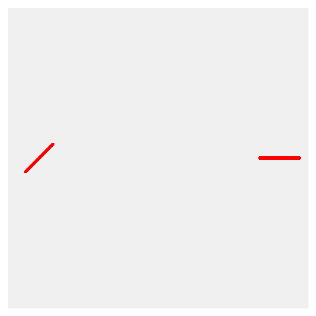
\includegraphics[width=1\linewidth]{2bars3}
\end{subfigure}%
\hfill
\begin{subfigure}{.5\textwidth}
  \centering
  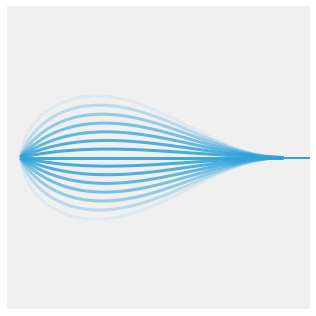
\includegraphics[width=1\linewidth]{2bars_2}
\end{subfigure}
\hfill
\begin{subfigure}{.5\textwidth}
  \centering
  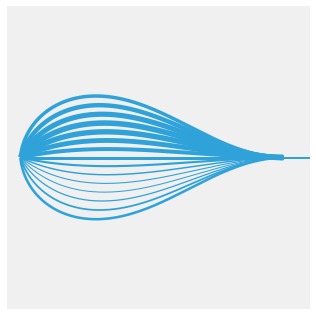
\includegraphics[width=1\linewidth]{2bars_1}
\end{subfigure}%
\hfill
\begin{subfigure}{.5\textwidth}
  \centering
  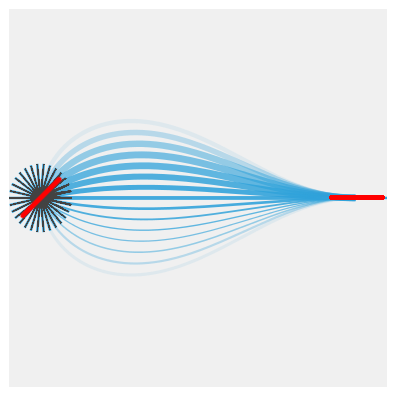
\includegraphics[width=1\linewidth]{2bars}
\end{subfigure}
\floatfoot{(Still figuring out how to make the plot clearer. Pop out effect. First column input, second column connections without torus, third column torus}
\end{figure}

\plotfigureS{2bars}{Experiment setup. Left red bar - center, right red bar - flanker, black bars - orientation selective neurons, blue curves - elastica curves. The position of the center bar is encoded by n orientation selective neurons. The modulation from the flanker is directly calculated from the orientation of the flanker bar, rather than through encoding it with orientation selective neurons. The more saturated the color, the stronger the connection between the orientation selective neuron and the flanker (not dependant on the presented center orientation). The wider the curve, the stronger the response of that neuron (dependent on the presented center orientation.}{Two bars setup}{0.5}
\plotfiguresix{el_ener}{h_add}{h_mul}{cen}{ad_comb}{mul_comb}{\bt{Additive and Multiplicative model} (a) Elastica energy (b) h, additive (c) h, multiplicative (d) Central drive (e) Final response for additive model (f) Final response for multiplicative model}{.49}{Additive and Multiplicative mode}
\plotfigure{ADD_vs_MULT}{Additive vs Multiplicative model. Although the tilt effects happen at different orientations and the strength of modulation is different, the change in the effect as we vary the flanker orientation is similar.}{AdMp}
\section{Passive vs Dynamic models}
%\subsection{Center and flanker bar}
\section{Tilt effects}

In this section we explore variety of tilt effects. In all of the experiments we have a center bar and a number of flanker bars around it. We experiment with different number of flankers, vary their position and orientation around the center bar.

\begin{figure}[H]
\caption{}
\begin{subfigure}{.5\textwidth}
  \centering
  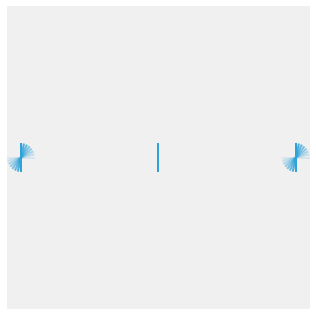
\includegraphics[width=0.5\linewidth]{fig5_B}
  \caption{}
\end{subfigure}%
\hfill
\begin{subfigure}{.5\textwidth}
  \centering
  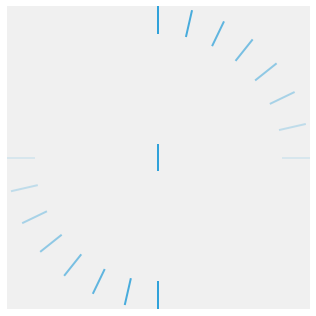
\includegraphics[width=0.5\linewidth]{fig5_C}
  \caption{}
\end{subfigure}
\hfill
\begin{subfigure}{.5\textwidth}
  \centering
  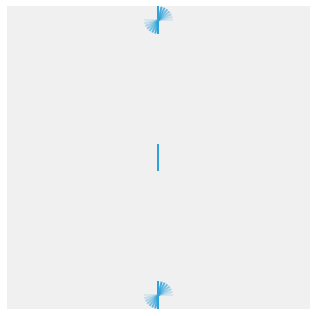
\includegraphics[width=0.5\linewidth]{fig5_D}
  \caption{}
\end{subfigure}%
\hfill
\begin{subfigure}{.5\textwidth}
  \centering
  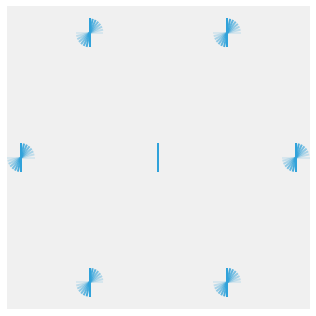
\includegraphics[width=0.5\linewidth]{fig5_F}
  \caption{}
\end{subfigure}
\floatfoot{Pop out effect. First column input, second column connections without torus, third column torus}
\end{figure}

\subsection{Tilt effect 1}
\plotfigureS{fig5_B}{Tilt Effect 1}{Tilt Effect 1}{0.3}
\plotfigureS{matrix}{Weight matrix}{Weight Matrix 1}{0.5}
(fix legend)
\plotthreefigures{p_cen}{d_cen}{d_flan}{Experienced tilt illusions for different modulation constants. (a) Tilt illusion of the center bar for different flaker orientations. The experiment reproduced is from \cite{keemink2015unified}, fig.5, B (b) Tilt illusion of the center bar for different flanker orientations, in the dynamic mode. (c) Tilt illusion of the flanker bars for different flanker orientations, in a dynamic model}{Experienced tilt illusions}{1}
\subsection{Tilt effect 2}
\plotfigureS{fig5_C}{Tilt Effect 2}{Tilt Effect 2}{0.3}
\subsection{Tilt effect 3}
\plotfigureS{fig5_D}{Tilt Effect 3}{Tilt Effect 3}{0.3}
\subsection{Tilt effect 4}
\plotfigureS{fig5_F}{Tilt Effect 4}{Tilt Effect 4}{0.3}

\section{Pop out effects}


\begin{figure}[H]
\caption{}
\begin{subfigure}{.33\textwidth}
  \centering
  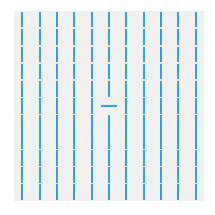
\includegraphics[width=1\linewidth]{bar}
\end{subfigure}%
\hfill
\begin{subfigure}{.33\textwidth}
  \centering
  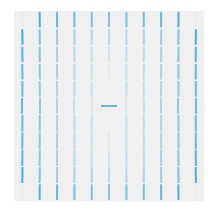
\includegraphics[width=1\linewidth]{bar_without}
\end{subfigure}
\hfill
\begin{subfigure}{.33\textwidth}
  \centering
  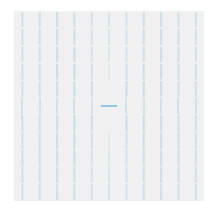
\includegraphics[width=1\linewidth]{bar_torus}
\end{subfigure}%
\hfill
\begin{subfigure}{.33\textwidth}
  \centering
  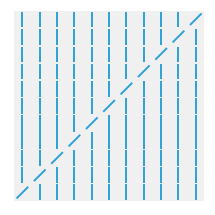
\includegraphics[width=1\linewidth]{line}
\end{subfigure}
\hfill
\begin{subfigure}{.33\textwidth}
  \centering
  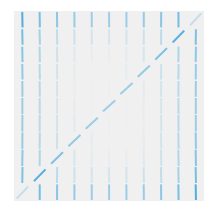
\includegraphics[width=1\linewidth]{line_without}
\end{subfigure}%
\hfill
\begin{subfigure}{.33\textwidth}
  \centering
  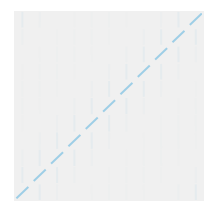
\includegraphics[width=1\linewidth]{line_torus}
\end{subfigure}
\hfill
\begin{subfigure}{.33\textwidth}
  \centering
  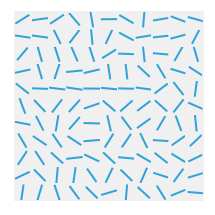
\includegraphics[width=1\linewidth]{random}
\end{subfigure}%
\hfill
\begin{subfigure}{.33\textwidth}
  \centering
  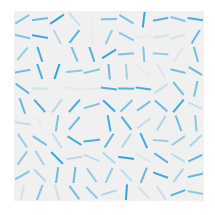
\includegraphics[width=1\linewidth]{random_without}
\end{subfigure}%
\hfill
\begin{subfigure}{.33\textwidth}
  \centering
  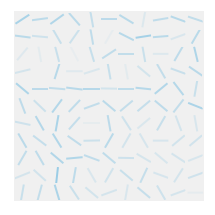
\includegraphics[width=1\linewidth]{random_torus}
\end{subfigure}
\floatfoot{Pop out effect. First column input, second column connections without torus, third column torus}
\end{figure}

\chapter{Evaluation}

\chapter{Timeline}
\begin{figure}
\caption{}
\begin{tikzpicture}[timespan={}]


% timespan={Day} -> now we have days as reference
% timespan={}    -> no label is displayed for the timespan
% default timespan is 'Week'%

\timeline[custom interval=true]{May, Jun, Jul, Aug, Sep, Nov, Oct, Dec, Jan, Feb, Mar}
% \timeline[custom interval=true]{3,...,9} -> i.e., from Day 3 to Day 9
% \timeline{8} -> i.e., from Week 1 to Week 8


% put here the phases
\begin{phases}
\initialphase{involvement degree=4.75cm,phase color=black}
\phase{between week=5 and 7 in 0.7,involvement degree=4cm, phase color=black}
\phase{between week=7 and 9 in 0.7,involvement degree=2cm, phase color=black}
\phase{between week=5 and 9 in 0.7,involvement degree=4cm, phase color=green}
\phase{between week=9 and 11 in 0.1,involvement degree=2.25cm}
\phase{between week=8 and 11 in 0.7,involvement degree=2.25cm ,phase color=blue!80!cyan}
\end{phases}

% put here the milestones
\addmilestone{at=phase-0.180,direction=90:1cm,text={Project allocation},text options={above}}
\addmilestone{at=phase-0.270,direction=270:1cm,text={Sensory Systems (MIT OpenCourseWare)},text options={below}}

\addmilestone{at=phase-1.130,direction=130:2cm,text={Literature review},text options={above}}
\addmilestone{at=phase-1.230,direction=230:1cm,text={Neural Computation},text options={below}}
\addmilestone{at=phase-1.290,direction=290:2cm,text={Machine Learning Practical},text options={below}}

\addmilestone{at=phase-2.100,direction=100:3cm,text={More literature review},text options={above}}
\addmilestone{at=phase-2.310,direction=310:3cm,text={Neural Information Processing},text options={below}}

\addmilestone{at=phase-3.170,direction=170:1cm,text={Started working on Matlab implementation},text options={above}}
\addmilestone{at=phase-3.140,direction=140:1cm,text={Visual fields},text options={above}}
\addmilestone{at=phase-3.120,direction=120:1cm,text={Tuning curves},text options={above}}
\addmilestone{at=phase-3.90,direction=90:1cm,text={Population coding},text options={above}}
\addmilestone{at=phase-3.60,direction=60:1cm,text={Simple Dynamics},text options={above}}
\addmilestone{at=phase-3.30,direction=30:1.5cm,text={Dynamics with weight matrix},text options={above}}
\addmilestone{at=phase-3.270,direction=270:0.5cm,text={Python implementation},text options={below}}
\addmilestone{at=phase-3.300,direction=300:0.5cm,text={Elastica principle},text options={below}}

\addmilestone{at=phase-4.120,direction=120:0.3cm,text={Matlab experiments},text options={above}}
\addmilestone{at=phase-4.310,direction=310:0.3cm,text={Python experiments},text options={below}}

\addmilestone{at=phase-5.140,direction=140:0.34cm,text={Interim report},text options={above}}
\addmilestone{at=phase-5.50,direction=50:0.34cm,text={Write},text options={above}}
\addmilestone{at=phase-5.330,direction=330:0.34cm,text={Write},text options={below}}
\addmilestone{at=phase-5.20,direction=20:1cm,text={Final write up},text options={above}}

\end{tikzpicture}
\label{timeline}
\floatfoot{\bt{Timeline of the project}\\\textcolor{gray}{Research}\\\textcolor{green}{Implementation}\\\textcolor{yellow}{Experiments}\\\textcolor{blue}{Write up}}
\end{figure}

Fig.\ref{timeline} illustrates the work I have done so far and my plan until end of march, when the final deadline for the report is. After the project was allocated to me, I spend some time during the summer watching online courses on neuroscience and sensory systems.

Beginning of the year, I took Neural Computation to get even more background. I started implementing all the necessary parts, in order to simulate the model - visual fields, tuning curves, population coding, etc. Afterwards I started implementing dynamics in the system, gradually extending the model. In my final model, I assume full connectivity between all the neurons. The connection at first are modeled based on the distance and difference in preferred orientations between them. My next goal is to incorporate the elastica principle into my model. 

At first I opted to use Matlab, as I had some experience with it. However with time, as I added some complexity to my model, I realized Matlab is not the base choice for the project. I decided to switch to Python, using Notebooks and Holoviews. Notebooks are a lot better way for structuring the code and write up at the same time. Holoviews was the other main reason, as it provides advanced plotting capabilities on multidimensional data, which is really viable when visualizing the output of recurrent neural networks for different time steps.


\chapter{Conclusions}

% use the following and \cite{} as above if you use BibTeX
% otherwise generate bibtem entries
\bibliographystyle{plain}
\bibliography{mybib}

\end{document}
